\chapter{Evaluation and results}
\label{chap:eval}

In the previous chapter, the evaluation suite and its features were presented.
This chapter is split into several subtopics.
First, it deals with the introduction of datasets.
Second, the quality metrics for the comparison of disparity algorithms  for stereoscopic videos are defined.
Third, the structure of the measurement is illustrated.
Fourth, the results are visualized and discussed.
\newline\newline\noindent Overall, the setup for the evaluation took 24 days to process 30 GB of stereoscopic videos and to create all disparity maps.
Accumulated, the computed disparity maps, the created masks as well as the heatmaps, took about 8 GB.

\section{Datasets}

A dataset basically describes a set of stereo images, which additionally contains ground-truth disparity maps.
The aim of such datasets is to provide accurate data, on which researchers can rely.
This datasets can be used to evaluate the performance of computer vision algorithms, such as disparity algorithms in this thesis.
Without having such datasets it would be crucial to rate the overall quality of for instance stereo matching algorithms.
As for today, no high-resolution stereoscopic video dataset yet exists, neither a synthetic nor a captured one.
In order to obtain ground-truth depth information, there exist in general two options.
On the one hand, the real-world can be sensed via area scanner, for instance a radar (cf. KITTI vision benchmark suite\footnote{\url{http://www.cvlibs.net/datasets/kitti/}}).
On the other hand, a synthetic computer-animated scene is generated and the renderer calculates the disparity.
Of course, the former approach is more error-prone than the latter one.
The former one can lack of accuracy due to false measurements whereas the latter one real ground-truth information provides.
\newline\newline\noindent \citeauthor{kondermann2015stereo} came up with an interesting approach.
As area scanners are never 100 percent accurate, they introduced error-bars, which can range from $0-10$.
An error-bar indicates how certain the area scanner was that this disparity for a given pixel really existed \citep{kondermann2015stereo}.
\newline\newline\noindent As it would be a tremendous task to evaluate every existing stereoscopic dataset with every existing disparity algorithms, here three different datasets were chosen.
\newline\newline\noindent Other datasets, which were found but not investigated are the MPI Sintel Stereo Training Data, created for optical flow evaluation \citep{Butler:ECCV:2012} and the Middlebury stereo dataset, providing real images with ground-truth information \citep{scharstein2006middlebury}.

\subsection*{Tsukuba stereo dataset}

As reference dataset, the reworked Tsukuba Stereo Dataset was chosen \citep{martull2012realistic}.
One of the three scenes is called tsukuba to honour the popular \textit{Head and Lamp} scene and was shortly introduced in the foundations Chapter \ref{chap:foundations}.
The reference dataset is used to see if the implementation leads to similar results as in other stereo benchmarks.
This does of course not verify that the presented implementation is error-free but can point in the right direction.
Of course, the settings (i.e. parameters of an algorithm) depends on the input material (e.g. size of the images, noise occurrences) and on the type of the scenery, for instance many regions with arbitrary surfaces (textured vs textureless).
Hence, it is possible to have good parameters for one scene and not for the other.
However, in order to evaluate those algorithms the reference dataset is used to see how the eval engine actually works with the same parameters on the same images.

\begin{figure}[h!]
\centering
\begin{tabular}{ccc}
\subfloat[tsukuba scene]{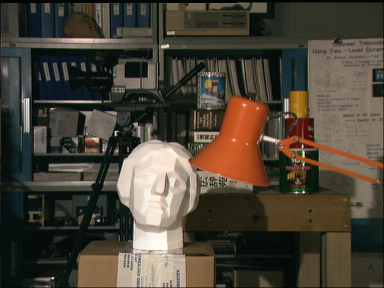
\includegraphics[width=0.3\textwidth]{src/images/tsukuba-imgL.png}} &
\subfloat[teddy scene]{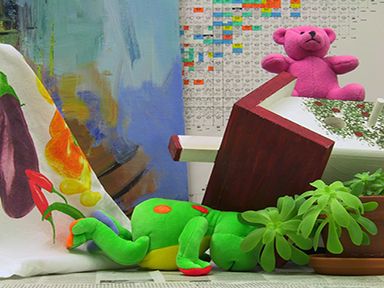
\includegraphics[width=0.3\textwidth]{src/images/teddy-imgL.png}} &
\subfloat[venus scene]{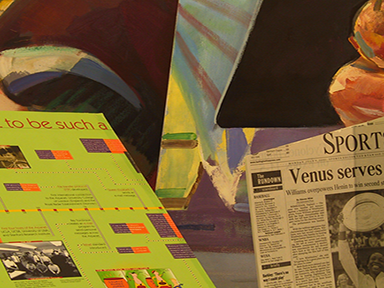
\includegraphics[width=0.3\textwidth]{src/images/venus-imgL.png}} \\
\subfloat[tsukuba disparity]{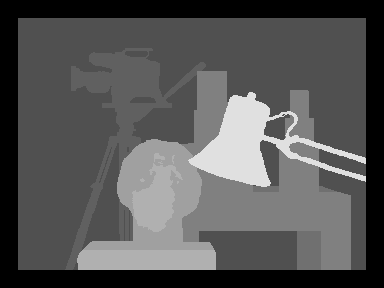
\includegraphics[width=0.3\textwidth]{src/images/tsukuba-dgt.png}} &
\subfloat[teddy disparity]{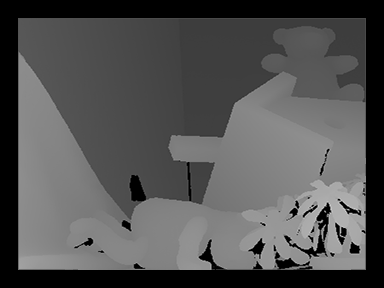
\includegraphics[width=0.3\textwidth]{src/images/teddy-dgt.png}} &
\subfloat[venus disparity]{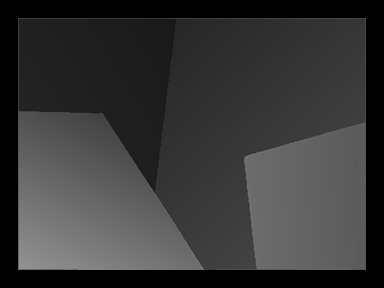
\includegraphics[width=0.3\textwidth]{src/images/venus-dgt.png}} \\
\end{tabular}
\caption[Tsukuba stereo dataset]{Tsukuba stereo dataset \citep{martull2012realistic}}
\label{fig:tsukuba2}
\end{figure}

\subsection*{Cambridge stereo dataset}

The second one is a dataset, especially created for the evaluation of the DCBGrid from the University of Cambridge\footnote{\url{http://www.cl.cam.ac.uk/research/rainbow/projects/dcbgrid/datasets/}}.
This is also one of the first stereoscopic dataset targeting videos.

\begin{figure}[h!]
  \centering
  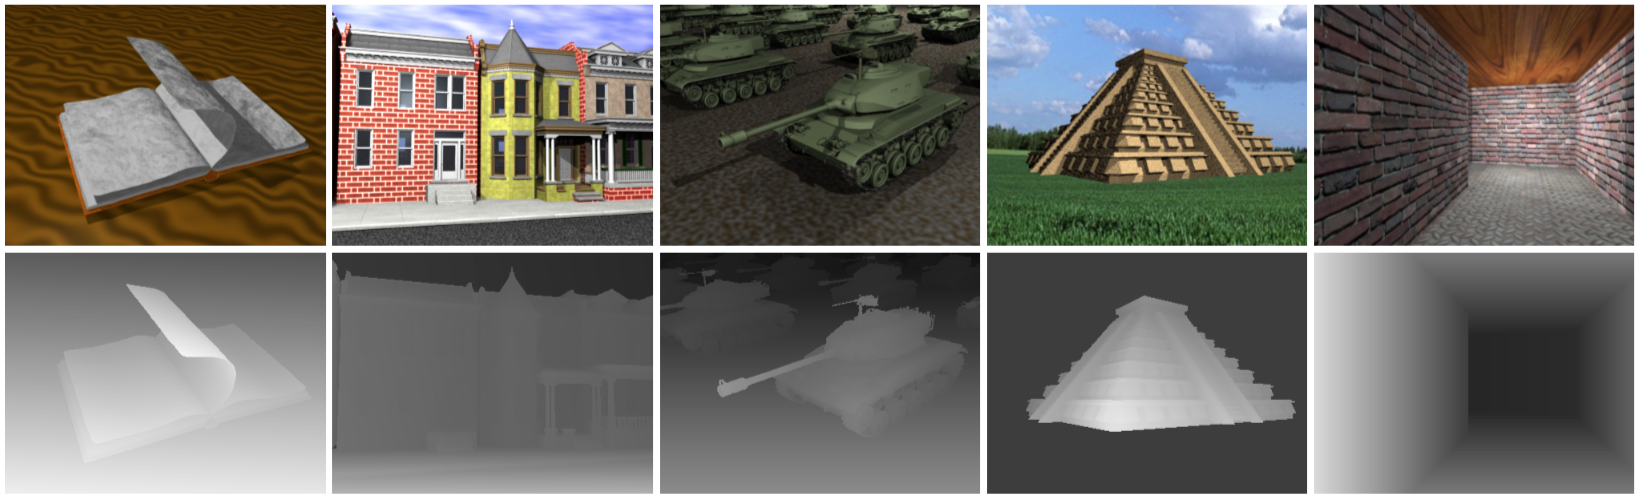
\includegraphics[width=1.0\textwidth]{src/images/dbcgrid-dataset.png}
  \caption[Middlebury stereo dataset example]{Middlebury stereo dataset example}
  \label{fig:dbcgrid-dataset}
\end{figure}

\noindent The Cambridge stereo dataset consists of five different rendered scenes in $400x300$ resolution with each about 100 frames \citep{richardt2010real}.
The dataset scales the disparity for each scene from $0$ to $64$.

\subsection*{SVDDD - a high-resolution Stereoscopic Video Dataset with precise Depth and Disparity information}

As third dataset, a novel, not yet analyzed dataset was chosen: the SVDDD\footnote{SVDDD stands for a high-resolution Stereoscopic Video Dataset with precise Depth and Disparity information.} dataset.
The Lehrstuhl f{\"u}r Praktische Informatik IV\footnote{\url{http://ls.fmi.uni-mannheim.de/de/pi4/}} created the dataset on its own with high-resolution video sequences containing accurate depth and disparity information for stereoscopic videos.
\newline\newline\noindent The difference here is, that this dataset was not analyzed before.
Thus, it is possible that the chosen algorithms work not properly on this dataset.
If this case occurs there exist two possibilities why this happens:

\begin{itemize}
  \item On the one hand, the disparity information are not properly calculated, or
  \item on the other hand, those algorithms have some troubles with the constructed scene.
\end{itemize}

\noindent Focusing on the latter one, the scenes were created with Blender and utilizes open-source scenes from the Big Buck Bunny project\footnote{\url{https://peach.blender.org}}.
A second camera was added to the scenes for obtaining depth information.
The parameter for each scene can be from the Blender files.
The scenes were also adjusted regarding the following points to deliver a certain value for stereo matching algorithms:

\begin{itemize}
  \item rays of light were removed,
  \item motion and object blur were reduced,
  \item fain-grained textures (like grass or hairs) were modified, and
  \item transparent layers were removed.
\end{itemize}

\noindent Otherwise, these points could lead to defective depth information.
The dataset consists of 15 scenes.
The scenes consist of high resolution stereo images $1920x1080$ with an average bitrate of 94 MBit/s.
With an approximate size of 2 MB for each frame, the size of each sequence varies between 0.4 GB and 2.7 GB.
For each frame, depth and disparity information are computed with 32-bit floating point precision and saved in OpenEXR files.

%todo add overview images

%explicit
\newpage

\section{Quality metrics}

Typical quality measure instruments for comparing disparity maps against their ground-truth reference data are  \citep{cyganek2011introduction}:

\begin{itemize}
  \item percentage of bad matching pixels,
  \item root-mean-square error,
  \item parameter-free measures.
\end{itemize}

\noindent As parameter-free measures needs modified disparity algorithms \citep{cyganek2011introduction}, it was not considered.

\subsection*{Percentage of bad matching pixels}

Percentage of bad matching pixels (PBMP) is usually used in comparing the performance of stereo matching algorithms.

\begin{equation}
  \operatorname{PBMP}=\frac{1}{n} \sum_{x,y=0}^{}(|d_a(x,y) - d_e(x,y)| > \delta_t)
\end{equation}

\noindent The threshold, denoted with $\delta_t$, can be adjusted and as result, the percentage of outlier pixels, which differ by more than $\delta_t$, is estimated.

\subsection*{Root-mean-squared error}

The mean squared error (MSE) as well as the root mean squared error (RMSE) are both the most popular metrics in image and video processing \citep{cyganek2011introduction, benoit2008quality, scharstein2002taxonomy}.
The MSE is, as the name implies, the mean of the squared differences between the intensities of pixels in two pictures at the same position.
In conclusion, the average difference per pixel is then the root of the squared error.

\begin{equation}
  \operatorname{RMS-Error}=\sqrt{\frac{1}{n} \sum_{x,y=0}^{}(d_a(x,y) - d_e(x,y))^2}
\end{equation}

\noindent It represents the sample standard deviation of the differences between predicted values and observed values.
Here $d_a(x,y)$ is the actual disparity value for given $x$ and $y$.
$d_e(x,y)$ is our expected disparity value from our ground-truth data.
Hence the RMSE is the difference between values on average.

\section{Measurement}



\subsection*{Parameter tuning}

Our results.
because there exist arbitrary combination for the OpenCV implementations.
The other drawback is that neither the implemented algorithms nor my own have the possibility of adjustments.

\subsection*{Visualization}

The results are visualized with heatmaps utilizing the OpenCV autumn scheme.

\begin{figure}[h!]
  \centering
  
\includegraphics[width=0.6\textwidth]{src/images/colorscale.png}
  \caption[OpenCV autumn color scale]{OpenCV autumn color scale\protect\footnotemark}
  \label{fig:colorscale}
\end{figure}
\footnotetext{Source (accessed 04/2016): \url{http://docs.opencv.org/3.1.0/d3/d50/group__imgproc__colormap.html}.}

%todo add opencv autumn scheme
%todo describe a bit the colouring

"The human perception isn't built for observing fine changes in grayscale images. Human eyes are more sensitive to observing changes between colors, so you often need to recolor your grayscale images to get a clue about them. OpenCV now comes with various colormaps to enhance the visualization in your computer vision application."

Outliers are marked with purple in the heatmaps.
The border is excluded from the evaluation (cf. Chapter \ref{chap:foundations}) and also marked purple.
The more heat, the brighter the color, the nearer the objects are.

\subsection*{Applying disparity algorithms on videos}

As said in the implementation Chapter \ref{chap:impl}, disparity algorithms for image can be applied to videos.
Although the frames of a video can be seen as independent pieces, different anomalies can be further investigated while analyzing videos:

\begin{itemize}
  \item outliers in the form of a single frames which differs too much from the others,
  \item impact of noise,
  \item the benefit from creating a naive spatiotemporal context.
\end{itemize}

\noindent The following sections present the results.

%explicit
\newpage
\section{Results}

%todo define abbreviations for tables
\noindent The following Table \ref{tab:metrics} contains all combinations of the presented masks with the established metrics.
As of now, the tags are used in upcoming descriptions and result tables.

\begin{table}[h!]
\centering
\begin{tabular}{l|l}
\textbf{Tag} & \textbf{Description} \\ \hline \hline
$\sigma_{0.6}$ & Gaussian noise with $\sigma$ of 0.6. \\ \hline
$\gamma_{28}$ & Applied H.265 compression with a CRF of 28. \\ \hline \hline
$\varepsilon_{all}$ & RMSE in complete image. \\ \hline
$\varepsilon_{noc}$ & RMSE in non-occluded regions. \\ \hline
$\varepsilon_{disc}$ & RMSE in depth-discontinuity regions. \\ \hline
$\varepsilon_{tex}$ & RMSE in textured regions. \\ \hline
$\varepsilon_{sal}$ & RMSE in salient regions. \\ \hline \hline
$\delta_{all}$ & PBMP in complete image. \\ \hline
$\delta_{noc}$ & PBMP in non-occluded regions. \\ \hline
$\delta_{disc}$ & PBMP in depth-discontinuity regions. \\ \hline
$\delta_{tex}$ & PBMP in textured regions. \\ \hline
$\delta_{sal}$ & PBMP in salient regions. \\ \hline
\end{tabular}
\caption{Overview on used metrics in upcoming result matrices.}
\label{tab:metrics}
\end{table}

%todo small intro


%todo results

%explicit
\newpage
\subsection{Against reference dataset}

As reference scene the \textit{Head and lamp} scene of the Tsukuba dataset was chosen.
For evaluating against the reference dataset, all presented disparity algorithms computed disparity maps.
These disparity maps are then compared in combination with different masks.
The result can be seen in Table \ref{tab:eval:snsm:tsukuba} and the SNSM is depict in Figure \ref{fig:eval:snsm:tsukuba}.
Compared with the Middlebury stereo benchmark\footnote{\url{http://vision.middlebury.edu/stereo/eval/}}, similar results could be achieved.
The SNSM utilizes SAD as matching cost function and does not further disparity refinement.
The results from SNSM with a threshold of $4$ and a block size of $9$ are $\delta_{all} = 6.78\%$ and $\varepsilon_{all} = 2.03px$.
According to the Middlebury stereo benchmark, the other SAD implementation (SAD-IGMCT) \citep{ambrosch2010accurate} achieved with a threshold of $2$: $\delta_{all} = 2.92\%$.
The difference comes from smoothing, which SAD-IGMCT included as a disparity refinement step, which is visible while looking at their outcome.

%todo add other algorithm outputs

\begin{figure}[h!]
\centering
\begin{tabular}{ccc}
\subfloat[ground-truth heatmap]{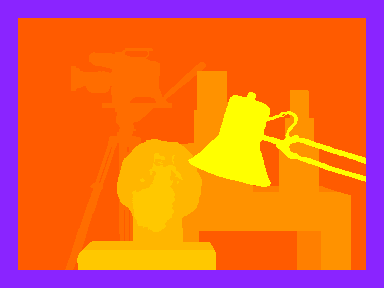
\includegraphics[width=0.45\textwidth]{src/images/evaluation/snsm-tsukuba-ground-truth.png}} &
\subfloat[computed disparity-map]{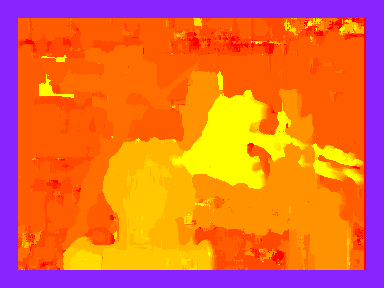
\includegraphics[width=0.45\textwidth]{src/images/evaluation/snsm-tsukuba-disparity-map.png}} \\
\subfloat[outliers in SNSM]{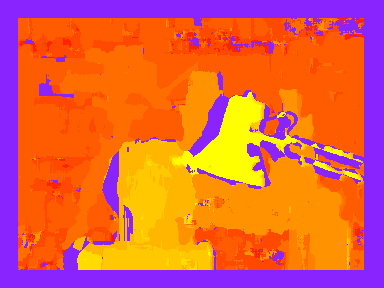
\includegraphics[width=0.45\textwidth]{src/images/evaluation/snsm-tsukuba-outliers.png}} &
\subfloat[outliers in SAD-IGMCT]{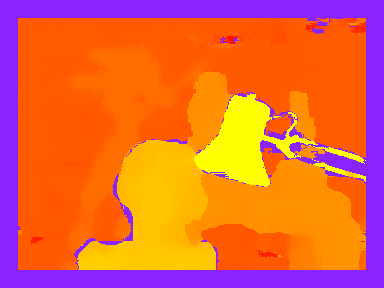
\includegraphics[width=0.45\textwidth]{src/images/evaluation/snsm-tsukuba-outliers-igmct.png}}
\end{tabular}
\caption{SNSM heatmaps for Tsukuba scene}
\label{fig:eval:snsm:tsukuba}
\end{figure}

\begin{table}[h!]
\centering
\begin{tabular}{l|rrrrrr}
  \hline
  \textbf{Method} & $\varepsilon_{all}$ & $\delta_{all}$ \\ \hline \hline
  SAD & $6.78\%$ & $2.03px$ \\ \hline
  SAD-IGMCT & $2.93\%$ & $1.38px$ \\ \hline
\end{tabular}
\caption{Result table for reference dataset}
\label{tab:eval:snsm:tsukuba}
\end{table}

\subsection{General performance}

\subsubsection{Simple stereo matcher}

\subsection{Impact of noise}

\subsubsection{Simple stereo matcher}

\subsection{Impact of video compression}

The impact of video compression is an interesting and novel approach.
High-resolution videos, due to its nature, are not shipped for television as uncompressed raw data or even lossless compressed.
As seen in the Chapter \ref{chap:related}, there are different applications for disparity algorithms.
One outpointed need is the remapping of disparity for different screen sizes.
If this can not happen on raw data, for instance the data is missing and only the compressed version is available, the influence of video compression on the outcome of disparity algorithms is observed.
\newline\newline\noindent For this observation five different datasets were created with the image diminisher.
As underlying video codec H.265 was chosen because it is currently the most efficient video compression technique.
The recommended default parameter for H.265, the constant rate factor (CRF) is 28.
It ranges from $0-51$, whereas 0 represents lossless and 51 the worst possible compression.
$0, 14, 28, 40, 51$ were chosen with $14$ and $40$ as additionally in-between parameters.
Thus, the observed range is $0, 14, 28, 40, 51$.

\subsubsection{Simple stereo matcher}

\subsection{Runtime}

\subsubsection{Simple stereo matcher}


\section{Discussion}

This is really important!


